
\section{Marco teórico}

\textbf{La importancia del aprendizaje de idiomas en un mundo globalizado: }Desde el siglo xix el idioma inglés se fue convirtiendo en un idioma obligado para las transacciones comerciales y de toda índole de negocios, tanto en los países desarrollados como en los del tercer mundo,  la globalización ha hecho de este idioma un lenguaje global, y este factor ha llevado a que sea incluido en negocios, cultura, e inclusive dentro de las aulas en países que no tienen este idioma \cite{ibm_pln} como lengua oficial. De este modo surge la necesidad de aprender una lengua extranjera que permita comunicarnos con otros países, y así poder derribar una barrera más entre la cultura y las relaciones internacionales de cada país.
\\
\\
\textbf{Teoría de la conectividad: }Es un modelo de aprendizaje que reconoce el cambio necesario de una sociedad en la que el aprendizaje ya no es una actividad individual, el impacto de las nuevas herramientas tecnológicas para la enseñanza de un lenguaje extranjero proporciona una mejoría en las habilidades de aprendizaje para los estudiantes.\cite{martinez2020herramientas}.
\\
\\
\textbf{El uso de la gamificación para procesos educativos: }La gamificación es la utilización de elementos de diseño de videojuegos en contextos que no son de juego, una técnica en orden de conseguir mejores resultados en el proceso de enseñanza-aprendizaje, posee elementos y técnicas propias de los juegos que se pueden explotar para poder facilitar la interiorización de conocimientos de una forma más divertida y llamativa. Dentro del ámbito del aprendizaje del inglés \cite{molina2021gamificacion}, la gamificación se convierte en una gran oportunidad para mejorar habilidades de expresión oral.
\\
\\
\textbf{Procesamiento de Lenguaje Natural (PLN) en la enseñanza de idiomas: }El procesamiento de lenguaje natural usa distintas reglas gramaticales y lingüísticas como tiempos gramaticales, sistemas semánticos, morfemas etc. Con el fin de desarrollar sistemas de software aplicados a un lenguaje en específico, es un proceso efectivo para asistir a los estudiantes en el proceso de aprendizaje científico, implementando \cite{alhawiti2014natural} PLN en el ámbito educacional no solo ayuda en el desarrollo efectivo del lenguaje, sino también a mejorar el rendimiento académico.Utilizando técnicas de procesamiento de lenguaje Natural se pueden desarrollar estrategias educacionales, que puedan asistir al buen aprendizaje y enseñanza.
\vfill
\subsection{Marco Conceptual}

\textbf{Competencia lingüística: }Habilidad esencial para comunicarse en un idioma, permitiendo la interacción efectiva en diversos contextos. Esta competencia implica no solo el dominio del vocabulario y la gramática, sino también la capacidad de comprender y expresar ideas de manera fluida y precisa \cite{martinez2020herramientas}.
\\
\\
\textbf{Hugginface: }
Hugging Face \cite{Jain2022} es una empresa franco-estadounidense fundada en 2016, reconocida por su contribución al desarrollo de herramientas de código abierto en el ámbito del aprendizaje automático y, en particular, del procesamiento de lenguaje natural (PLN). Su plataforma proporciona una amplia gama de recursos, incluyendo modelos preentrenados, conjuntos de datos y bibliotecas que facilitan la implementación y despliegue de aplicaciones de inteligencia artificial. Entre sus productos más destacados se encuentra la biblioteca Transformers, que ofrece implementaciones de modelos de vanguardia como BERT y GPT, permitiendo a investigadores y desarrolladores acceder y utilizar estas tecnologías de manera eficiente.
\\
\\
\textbf{Procesamiento del lenguaje natural (PLN): } Se refiere a una parte de la inteligencia artificial que se ocupa en dar a las computadoras la capacidad de comprender textos y palabras habladas de la misma manera que los seres humanos, combina la lingüística computacional con modelos estadísticos, con el fin de permitir a las computadoras procesar el lenguaje humano \cite{ibm_pln} en forma de texto, datos o datos de voz, para comprender su significado completo.
\\
\\
\textbf{SQuAD: } (Stanford Question Answering Dataset) es un conjunto de datos de comprensión lectora desarrollado por la Universidad de Stanford. Consiste en preguntas formuladas por trabajadores sobre un conjunto de artículos de Wikipedia, donde la respuesta a cada pregunta es un segmento de texto del pasaje correspondiente. Este conjunto de datos se utiliza ampliamente para entrenar y evaluar sistemas de respuesta a preguntas en el campo del procesamiento de lenguaje natural \cite{Rajpurkar2016}.
\\
\\
\textbf{RACE: } (ReAding Comprehension from Examinations) es un conjunto de datos de comprensión lectora a gran escala, recopilado de exámenes de inglés diseñados para estudiantes de secundaria en China. El conjunto consta de aproximadamente 28,000 pasajes y cerca de 100,000 preguntas generadas por expertos humanos (profesores de inglés), cubriendo una variedad de temas cuidadosamente diseñados para evaluar la capacidad de comprensión y razonamiento de los estudiantes. Ademas la alta proporción de preguntas que requieren razonamiento, lo que lo convierte en un recurso valioso para la investigación y evaluación en comprensión de lectura automática \cite{Lai2017}.
\\
\\
\textbf{Word2Vec: } Word2Vec es una técnica desarrollada por Mikolov et al. en 2013 que utiliza redes neuronales para aprender representaciones vectoriales de palabras a partir de grandes corpus de texto \cite{mikolov2013}.
\\
\\
\textbf{GloVe: } (Global Vectors for Word Representation) es un modelo desarrollado por Pennington et al. en 2014 que combina las ventajas de los modelos basados en conteo global y los modelos predictivos como Word2Vec. Construye una matriz de coocurrencia de palabras a partir de un corpus y aprende representaciones vectoriales que capturan las relaciones de coocurrencia entre palabras \cite{Pennington2014}.
\\
\\
\newpage
\textbf{Transformadores: } Son una arquitectura de red neuronal diseñada para procesar datos secuenciales, como texto o audio, mediante un mecanismo llamado atención. Este mecanismo permite al modelo enfocarse en diferentes partes de la entrada simultáneamente, capturando relaciones contextuales a largo plazo. \cite{vaswani2023attentionneed}.
\\
\\
\textbf{word embeddings:} Son representaciones numéricas de palabras en un espacio vectorial. En lugar de tratar las palabras como entidades aisladas, los word embeddings las representan como vectores de números reales, permitiendo que palabras con significados similares tengan representaciones cercanas en este espacio \cite{wordembeddingssurvey}.

\begin{figure}[h]
  \centering
  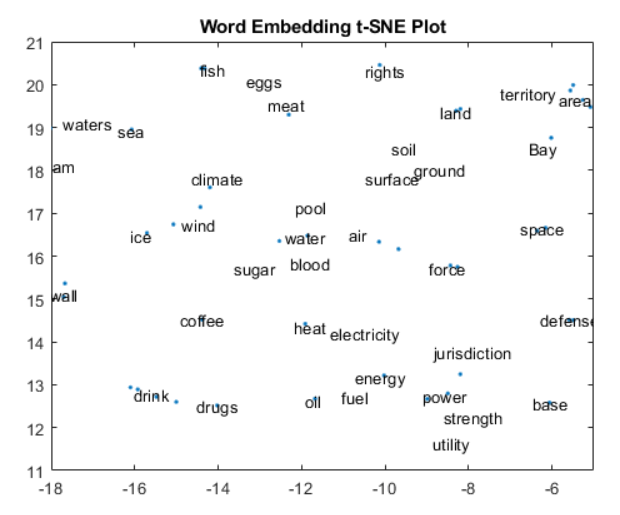
\includegraphics[width=0.5\linewidth]{Imagenes/word emmbedings.png}
  \caption{Representación de Word Emmbedings}
  Fuente: Visualize word embeddings \cite{mathworks1}
  \label{fig:word_emmbedings}
\end{figure}

\newpage
\textbf{GPT: Generative Pre-trained Transformer}

Este modelo utiliza una arquitectura de transformadores centrada exclusivamente en el decodificador unidireccional, lo que le permite generar texto de manera auto regresiva, prediciendo cada palabra basándose únicamente en las palabras anteriores en la secuencia.

\begin{figure}[H]
  \centering
  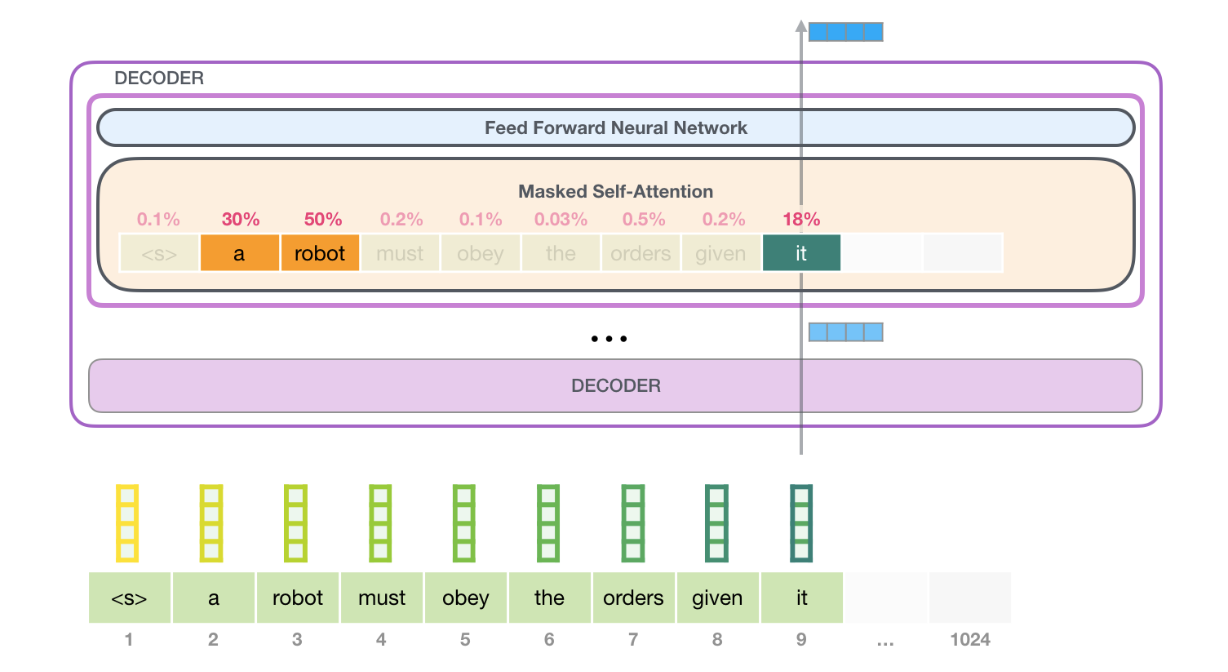
\includegraphics[width=0.8\linewidth]{Imagenes/gpt mascara de atencion.png}
  \caption{Arquitectura de GPT-2.}
  Fuente: The illustrated gpt-2 \cite{alammar2018gpt2}.
  \label{fig:gpt2_flow}
\end{figure}


La Fig.~\ref{fig:gpt2_flow} muestra el flujo interno de GPT-2:
\begin{itemize}
  \item Cada token de entrada (en la parte inferior) se convierte en un embedding posicional y se alimenta al primer bloque \emph{decoder}.
    \item Dentro de cada bloque \emph{Decoder}, la operación de \emph{Masked Self-Attention} evita que el modelo “mire” palabras que aún no han sido generadas. Es decir, cuando GPT-2 está prediciendo el token $t$, esta capa solo le permite revisar la información de los tokens anteriores (1, 2, ..., $t-1$), bloqueando cualquier dato posterior a $t$. De este modo, el modelo aprende a generar cada palabra basándose únicamente en el contexto previo, sin filtrar información del futuro, lo cual garantiza que la predicción sea verdaderamente auto-regresiva.

  \item Después de la atención, una red (barra celeste) refina la representación antes de pasarla al siguiente bloque.
  \item Tras apilar varias capas de este tipo (rectángulos lila), el nivel superior proyecta la salida en logits sobre el vocabulario y escoge la palabra más probable.  
\end{itemize}

\newpage
\textbf{BERT: } (Bidirectional Encoder Representations from Transformers), propuesto por Devlin et al. en 2019, es un modelo basado en transformadores que se pre-entrena en grandes corpus de texto. La bidireccionalidad de BERT permite que cada token considere el contexto completo en ambas direcciones, mejorando la comprensión del lenguaje.

\begin{figure}[H]
  \centering
  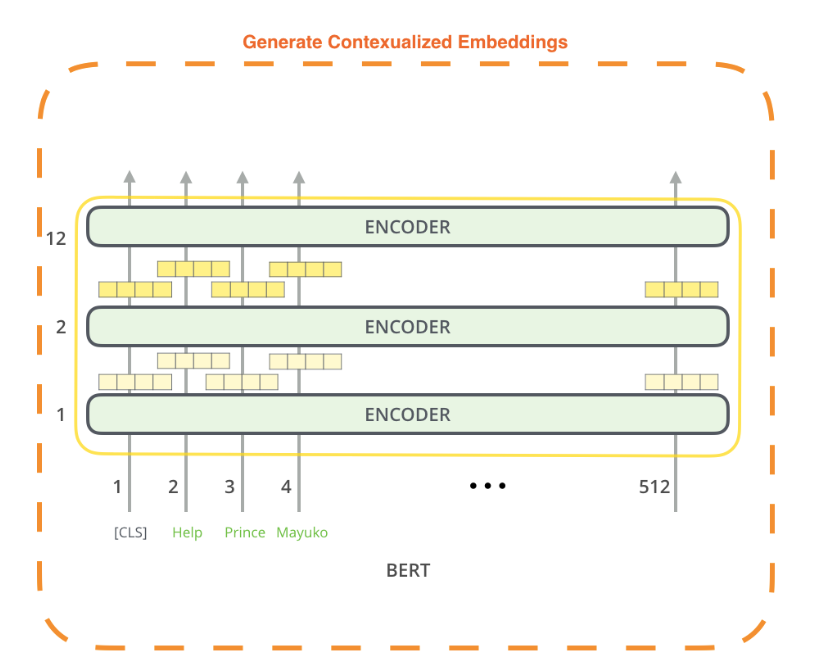
\includegraphics[width=0.8\textwidth]{Imagenes/arquitectura_bert.png}
  \caption{Arquitectura de BERT base}
   Fuente: The illustrated BERT \cite{alammar2018bert}.
  \label{fig:bert_architecture}
\end{figure}

La Fig.~\ref{fig:bert_architecture} muestra el flujo interno de BERT en donde:

\begin{itemize}

    \item BERT toma una secuencia de tokens que incluye un token especial de clasificación \texttt{[CLS]} seguido de tokens como "Help", "Prince", y "Mayuko".

    \item BERT base utiliza 12 capas de encoders (codificadores) para procesar los tokens. Cada capa aplica atención bidireccional, permitiendo que cada token considere el contexto completo de los otros tokens dentro de la secuencia (es decir, tanto antes como después del token a predecir).

    \item A medida que los tokens atraviesan las capas de encoders, se generan representaciones de salida para cada uno. Esto contribuye a la capacidad de BERT para contextualizar palabras y proporcionar representaciones ricas en significado, útiles para diversas tareas de procesamiento de lenguaje natural.

\end{itemize}

\textbf{T5: }(Text-to-Text Transfer Transformer), es un modelo de tipo encoder-decoder basado en la arquitectura Transformer. Su principal innovación es tratar todas las tareas de procesamiento de lenguaje natural (PLN) como problemas de entrada y salida de texto (text-to-text).

\begin{figure}[H]
  \centering
  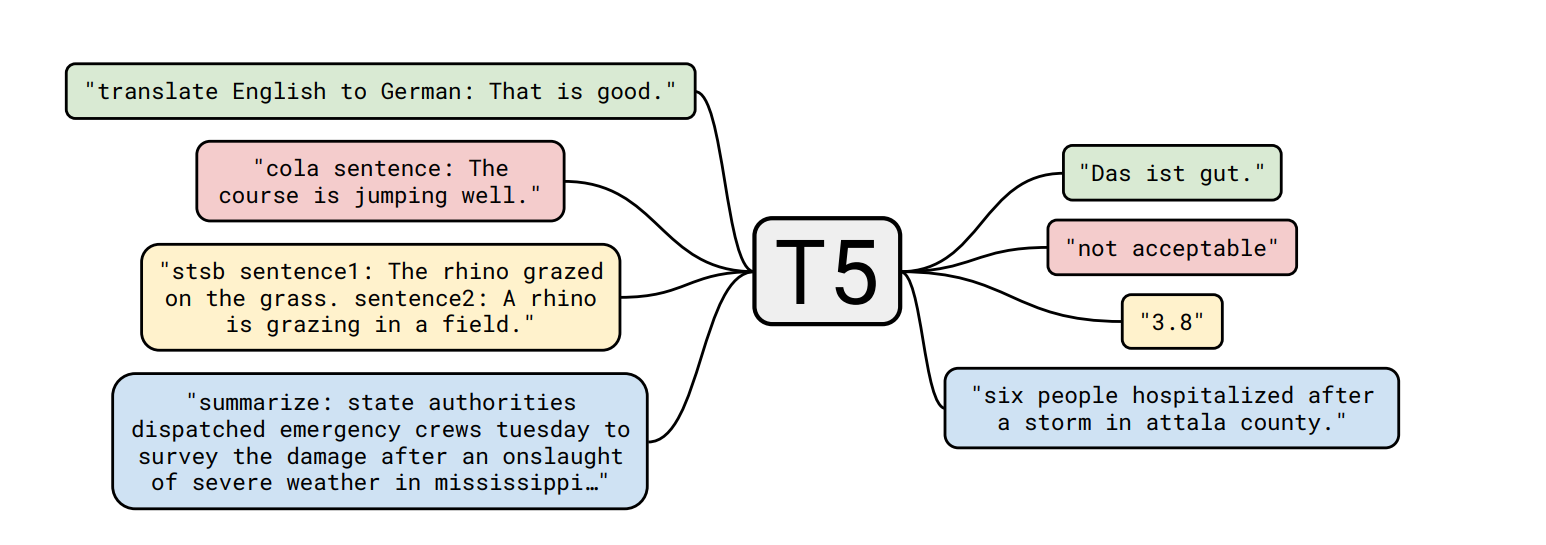
\includegraphics[width=0.7\linewidth]{Imagenes/t5.png}
  \caption{Representación gráfica t5}
  Fuente: Exploring the limits of t5 \cite{transferttt}
  \label{fig:t5_summary}
\end{figure}

\textbf{Inteligencia artificial: } Es un campo que combina la informática y conjuntos de datos robustos para permitir la resolución de problemas, engloba los subcampos del aprendizaje automático y el aprendizaje profundo \cite{ibm_ia} compuestos por algoritmos matemáticos, con el fin de hacer que la computadora “piense” por sí sola, y si realiza predicciones clasificaciones basadas en datos de entrada (preprocesamiento de datos).
\\
\\
\textbf{perplejidad: }
La perplejidad cuantifica la incertidumbre de un modelo al predecir la siguiente palabra en una secuencia. Matemáticamente, se define como la exponencial de la entropía cruzada promedio negativa \cite{huggperplexity}.

\textbf{Gamificación: } El concepto de gamificación consiste en el uso de elementos de juego en contextos no lúdicos. Se basa en el éxito de la industria de los videojuegos, las redes sociales y décadas de investigación en psicología humana, con el fin de aumentar la participación y motivación del usuario en un contexto dado \cite{flores2015using}. Además, la gamificación crea en los usuarios una sensación de compromiso a medida que avanzan en la realización de procesos y la finalización de tareas.
\\
\\
\textbf{Aplicación web: } Es un software que se ejecuta en el navegador web y es accesible desde diferentes dispositivos, ya sean personales o empresariales. Sin embargo, no se descarga en el dispositivo; se ejecuta en un servidor que se comunica a través de internet para, finalmente, llegar al navegador web que está realizando la petición \cite{aws_webapp}.
